\begin{figure}[]
	\centering
	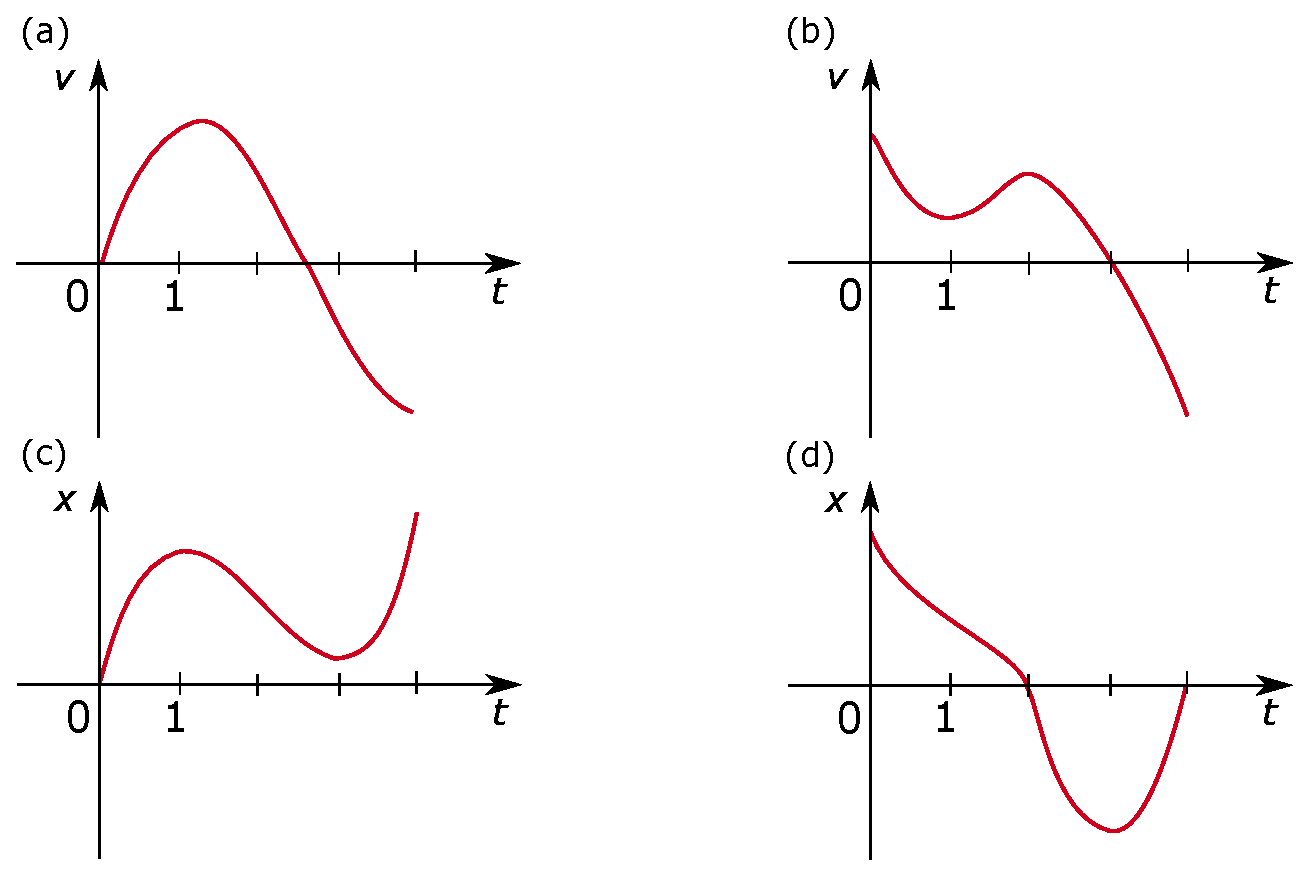
\includegraphics[width=0.65\textwidth]{Matematik/matfig/vx_grafer.eps}
	\caption{Hastighed og position som funktion af tiden.}
	\label{fig:vx_grafer}
\end{figure}
%%
\subsection*{Differentialregning}
%%
\begin{opgave}[1]{Hastighed og postion}
	\opg Figur \ref{fig:vx_grafer} (a) og (b) viser hastigheden af to objekter som funktion af tiden i sekunder. Hvornår sætter de to objekter hastigheden op, og hvornår sætter de hastigheden ned? Forklar dit svar.
	\opg Figur \ref{fig:vx_grafer} (c) og (d) viser positionen af to objekter $x$ som funktion af tiden i sekunder. Hvornår sætter de to objekter hastigheden op, og hvornår sætter de hastigheden ned? Forklar dit svar.
\end{opgave}
%%
%%
\begin{opgave}[2]{Afledede og dobbeltafledede}
Find den afledede og dobbeltafledede med hensyn til $x$ for følgende funktioner:
\opg $f(x) = x^2 + 4x.$
\opg $f(x) = \dfrac{1}{x} + \dfrac{1}{x^2}.$
\opg $f(x) = \cos(x).$
\opg $f(x) = \ln(x).$
\opg $f(x) = x \sin(x).$
\opg $f(x) = \dfrac{1}{x} \ln(x).$
\end{opgave}
%%
%%
\begin{opgave}[2]{Sammensatte funktioner}
Skriv følgende udtryk som en sammensat funktion $f(g(x))$ (altså skal du identificere den indre funktion $g(x)$ og den ydre funktion $f(g)$). Beregn derefter $\dv*{f}{x}$.\\ 
\opg $f(x) = \sin (4x).$
\opg $f(x) = \sqrt{2x}.$
\opg $f(x) = \sqrt{4x+5}.$
\opg $f(x) = \sin(e^x).$
\opg $f(x) =  \ln \left( \cos x \right).$
\end{opgave}
%%
%%
\begin{opgave}[3]{Funktioner af flere variable -- partiel differentiering}
I denne opgave skal vi kigge på partiel differentiering og kigger som et eksempel på funktioner af tre variable $f(x,y,z)$. For hver af de følgende funktioner skal I beregne den partielt afledede ift. både $x$, $y$ og $z$.
\opg $f(x,y,z) = x +y^2 + z^3.$
\opg $f(x,y,z) = x y^2 +  ye^{-z}.$
\opg $f(x,y,z) = ze^{xyz}.$
\opg $f(x,y,z) = \dfrac{x-y+5z}{x+y+z}.$ \\
\end{opgave}
%%